\documentclass[tikz,border=20pt]{standalone}
\usepackage{amsmath, amssymb}
\usetikzlibrary{matrix, positioning, fit, backgrounds, calc}

\begin{document}
	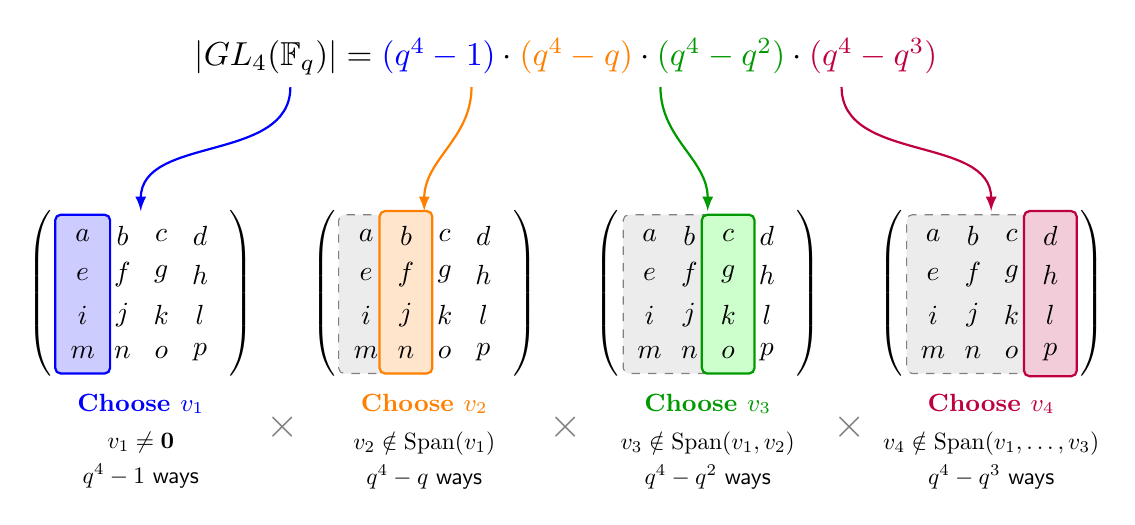
\begin{tikzpicture}[
		font=\sffamily,
		% Style for the 4x4 matrices
		mtx/.style={
			matrix of math nodes,
			left delimiter=(, right delimiter=),
			nodes={minimum width=1.2em, inner sep=2pt, anchor=center},
			column sep=2pt, row sep=2pt,
			ampersand replacement=\&
		},
		% Highlighting styles for active columns
		hl-v1/.style={fill=blue!20, draw=blue, thick, rounded corners=2pt},
		hl-v2/.style={fill=orange!20, draw=orange, thick, rounded corners=2pt},
		hl-v3/.style={fill=green!20, draw=green!60!black, thick, rounded corners=2pt},
		hl-v4/.style={fill=purple!20, draw=purple, thick, rounded corners=2pt},
		% Style for the forbidden "Span" subspace
		hl-span/.style={fill=gray!15, draw=gray, dashed, rounded corners=2pt},
		% Connector styles
		arrow/.style={->, >=latex, thick},
		term label/.style={font=\bfseries\small, align=center}
		]
		
		% --- 1. The Main Equation ---
		\node[scale=1.2] (eq) at (0, 0) {
			$|GL_4(\mathbb{F}_q)| = \textcolor{blue}{(q^4 - 1)} \cdot \textcolor{orange}{(q^4 - q)} \cdot \textcolor{green!60!black}{(q^4 - q^2)} \cdot \textcolor{purple}{(q^4 - q^3)}$
		};
		
		% Base node for vertical spacing
		\node[below=2.5cm of eq] (center_node) {};
		
		% --- 2. Branch 1: Column 1 (v1) ---
		\matrix[mtx, scale=0.85] (M1) at ($(center_node)+(-5.4, 0)$) {
			a \& b \& c \& d \\
			e \& f \& g \& h \\
			i \& j \& k \& l \\
			m \& n \& o \& p \\
		};
		\begin{scope}[on background layer]
			\node[hl-v1, fit=(M1-1-1)(M1-4-1)] {};
		\end{scope}
		\node[below=0.1cm of M1, term label, text=blue] {Choose $v_1$};
		\node[below=0.6cm of M1, scale=0.85, align=center] {$v_1 \neq \mathbf{0}$ \\[1mm] \textbf{$q^4 - 1$} ways};
		
		% --- 3. Branch 2: Column 2 (v2) ---
		\matrix[mtx, scale=0.85] (M2) at ($(center_node)+(-1.8, 0)$) {
			a \& b \& c \& d \\
			e \& f \& g \& h \\
			i \& j \& k \& l \\
			m \& n \& o \& p \\
		};
		\begin{scope}[on background layer]
			% Highlight the span of previous columns
			\node[hl-span, fit=(M2-1-1)(M2-4-1)] {};
			% Highlight current column
			\node[hl-v2, fit=(M2-1-2)(M2-4-2)] {};
		\end{scope}
		\node[below=0.1cm of M2, term label, text=orange] {Choose $v_2$};
		\node[below=0.6cm of M2, scale=0.85, align=center] {$v_2 \notin \mathrm{Span}(v_1)$ \\[1mm] \textbf{$q^4 - q$} ways};
		
		% --- 4. Branch 3: Column 3 (v3) ---
		\matrix[mtx, scale=0.85] (M3) at ($(center_node)+(1.8, 0)$) {
			a \& b \& c \& d \\
			e \& f \& g \& h \\
			i \& j \& k \& l \\
			m \& n \& o \& p \\
		};
		\begin{scope}[on background layer]
			\node[hl-span, fit=(M3-1-1)(M3-4-2)] {};
			\node[hl-v3, fit=(M3-1-3)(M3-4-3)] {};
		\end{scope}
		\node[below=0.1cm of M3, term label, text=green!60!black] {Choose $v_3$};
		\node[below=0.6cm of M3, scale=0.85, align=center] {$v_3 \notin \mathrm{Span}(v_1, v_2)$ \\[1mm] \textbf{$q^4 - q^2$} ways};
		
		% --- 5. Branch 4: Column 4 (v4) ---
		\matrix[mtx, scale=0.85] (M4) at ($(center_node)+(5.4, 0)$) {
			a \& b \& c \& d \\
			e \& f \& g \& h \\
			i \& j \& k \& l \\
			m \& n \& o \& p \\
		};
		\begin{scope}[on background layer]
			\node[hl-span, fit=(M4-1-1)(M4-4-3)] {};
			\node[hl-v4, fit=(M4-1-4)(M4-4-4)] {};
		\end{scope}
		\node[below=0.1cm of M4, term label, text=purple] {Choose $v_4$};
		\node[below=0.6cm of M4, scale=0.85, align=center] {$v_4 \notin \mathrm{Span}(v_1, \dots, v_3)$ \\[1mm] \textbf{$q^4 - q^3$} ways};
		
		% --- 6. Arrows linking equation to matrices ---
		\draw[arrow, blue] ($(eq.south)+(-3.5,0)$) to[out=270, in=90] (M1.north);
		\draw[arrow, orange] ($(eq.south)+(-1.2,0)$) to[out=270, in=90] (M2.north);
		\draw[arrow, green!60!black] ($(eq.south)+(1.2,0)$) to[out=270, in=90] (M3.north);
		\draw[arrow, purple] ($(eq.south)+(3.5,0)$) to[out=270, in=90] (M4.north);
		
		% --- 7. Multiplication Signs ---
		\node[scale=1.5, text=gray] at ($(M1)!0.5!(M2)+(0,-1.7)$) {$\times$};
		\node[scale=1.5, text=gray] at ($(M2)!0.5!(M3)+(0,-1.7)$) {$\times$};
		\node[scale=1.5, text=gray] at ($(M3)!0.5!(M4)+(0,-1.7)$) {$\times$};
		
	\end{tikzpicture}
\end{document}